% Options for packages loaded elsewhere
\PassOptionsToPackage{unicode}{hyperref}
\PassOptionsToPackage{hyphens}{url}
%
\documentclass[
]{article}
\usepackage{lmodern}
\usepackage{amssymb,amsmath}
\usepackage{ifxetex,ifluatex}
\ifnum 0\ifxetex 1\fi\ifluatex 1\fi=0 % if pdftex
  \usepackage[T1]{fontenc}
  \usepackage[utf8]{inputenc}
  \usepackage{textcomp} % provide euro and other symbols
\else % if luatex or xetex
  \usepackage{unicode-math}
  \defaultfontfeatures{Scale=MatchLowercase}
  \defaultfontfeatures[\rmfamily]{Ligatures=TeX,Scale=1}
\fi
% Use upquote if available, for straight quotes in verbatim environments
\IfFileExists{upquote.sty}{\usepackage{upquote}}{}
\IfFileExists{microtype.sty}{% use microtype if available
  \usepackage[]{microtype}
  \UseMicrotypeSet[protrusion]{basicmath} % disable protrusion for tt fonts
}{}
\makeatletter
\@ifundefined{KOMAClassName}{% if non-KOMA class
  \IfFileExists{parskip.sty}{%
    \usepackage{parskip}
  }{% else
    \setlength{\parindent}{0pt}
    \setlength{\parskip}{6pt plus 2pt minus 1pt}}
}{% if KOMA class
  \KOMAoptions{parskip=half}}
\makeatother
\usepackage{xcolor}
\IfFileExists{xurl.sty}{\usepackage{xurl}}{} % add URL line breaks if available
\IfFileExists{bookmark.sty}{\usepackage{bookmark}}{\usepackage{hyperref}}
\hypersetup{
  hidelinks,
  pdfcreator={LaTeX via pandoc}}
\urlstyle{same} % disable monospaced font for URLs
\usepackage{longtable,booktabs}
% Correct order of tables after \paragraph or \subparagraph
\usepackage{etoolbox}
\makeatletter
\patchcmd\longtable{\par}{\if@noskipsec\mbox{}\fi\par}{}{}
\makeatother
% Allow footnotes in longtable head/foot
\IfFileExists{footnotehyper.sty}{\usepackage{footnotehyper}}{\usepackage{footnote}}
\makesavenoteenv{longtable}
\usepackage{graphicx,grffile}
\makeatletter
\def\maxwidth{\ifdim\Gin@nat@width>\linewidth\linewidth\else\Gin@nat@width\fi}
\def\maxheight{\ifdim\Gin@nat@height>\textheight\textheight\else\Gin@nat@height\fi}
\makeatother
% Scale images if necessary, so that they will not overflow the page
% margins by default, and it is still possible to overwrite the defaults
% using explicit options in \includegraphics[width, height, ...]{}
\setkeys{Gin}{width=\maxwidth,height=\maxheight,keepaspectratio}
% Set default figure placement to htbp
\makeatletter
\def\fps@figure{htbp}
\makeatother
\usepackage[normalem]{ulem}
% Avoid problems with \sout in headers with hyperref
\pdfstringdefDisableCommands{\renewcommand{\sout}{}}
\setlength{\emergencystretch}{3em} % prevent overfull lines
\providecommand{\tightlist}{%
  \setlength{\itemsep}{0pt}\setlength{\parskip}{0pt}}
\setcounter{secnumdepth}{-\maxdimen} % remove section numbering

\date{}

\begin{document}

\hypertarget{markdown-cheatsheet}{%
\section{Markdown Cheatsheet}\label{markdown-cheatsheet}}

\hypertarget{text}{%
\subsection{Text}\label{text}}

\begin{verbatim}
# This is an <h1> tag
## This is an <h2> tag
###### This is an <h6> tag
\end{verbatim}

\emph{This text will be italic}\\
\emph{This will also be italic}\\
\textbf{This text will be bold}\\
\textbf{This will also be bold}\\
\emph{You \textbf{can} combine them}

\begin{verbatim}
*This text will be italic*  
_This will also be italic_  
**This text will be bold**  
__This will also be bold__  
*You **can** combine them*
\end{verbatim}

As Grace Hopper said: \textgreater{} I've always been more interested
\textgreater{} in the future than in the past.

\begin{verbatim}
As Grace Hopper said:  

> I’ve always been more interested
> in the future than in the past.
\end{verbatim}

Strikethrough \sout{text} here.

\begin{verbatim}
Strikethrough ~~text~~ here.
\end{verbatim}

http://github.com - automatic!

\href{http://github.com}{GitHub}

\href{mailto:CEMstudentexperience@dmu.ac.uk}{\nolinkurl{CEMstudentexperience@dmu.ac.uk}}

\begin{verbatim}
http://github.com - automatic!

[GitHub](http://github.com)

[CEMstudentexperience@dmu.ac.uk](mailto:CEMstudentexperience@dmu.ac.uk)
\end{verbatim}

\hypertarget{images}{%
\subsection{Images}\label{images}}

\begin{figure}
\centering

\includegraphics{https://www.dropbox.com/s/71r1lkrzihjl4fn/DMU-Logo-768x329.png?raw=1}
\caption{DMU logo}
\end{figure}

\begin{figure}
\centering
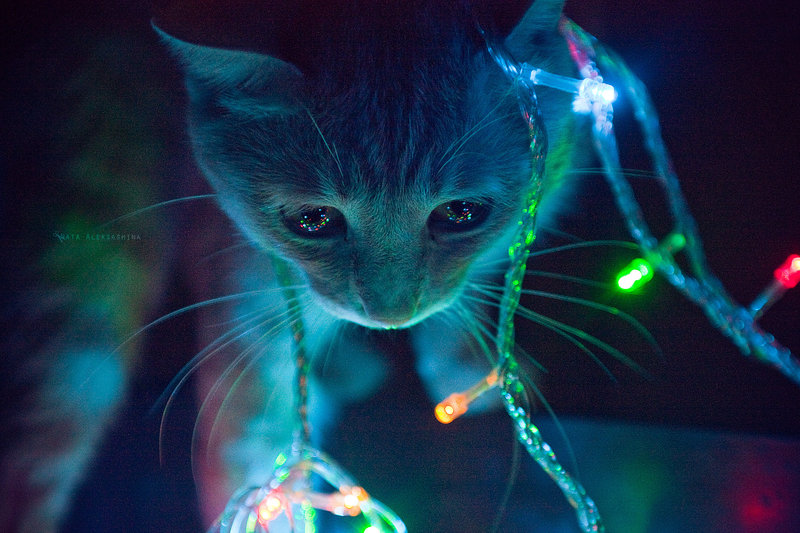
\includegraphics{technokitten.jpg}
\caption{cat}
\end{figure}

\begin{verbatim}
![alt](absolute url)
![alt](relative url)
\end{verbatim}

\hypertarget{tables}{%
\subsection{Tables}\label{tables}}

\begin{longtable}[]{@{}lr@{}}
\toprule
\endhead
Module Name: & \textbf{Multimedia III}\tabularnewline
Module Code: & \textbf{TECH3015}\tabularnewline
Title of Assessment: & \textbf{Coursework 1}\tabularnewline
This coursework item is: & \textbf{Summative /
\sout{Formative}}\tabularnewline
\bottomrule
\end{longtable}

\begin{verbatim}
|                          |                                |
|:-------------------------|-------------------------------:|
| Module Name:             | **Multimedia III**             | 
| Module Code:             | **TECH3015**                   |
| Title of Assessment:     | **Coursework 1**               |
| This coursework item is: | **Summative / ~~Formative~~**  |
\end{verbatim}

or

\begin{longtable}[]{@{}ll@{}}
\toprule
First Header & Second Header\tabularnewline
\midrule
\endhead
Content cell 1 & Content cell 2\tabularnewline
Content column 1 & Content column 2\tabularnewline
\bottomrule
\end{longtable}

\begin{verbatim}
First Header     | Second Header
---------------- | -------------
Content cell 1   | Content cell 2
Content column 1 | Content column 2
\end{verbatim}

\hypertarget{lists}{%
\subsection{Lists}\label{lists}}

\begin{itemize}
\tightlist
\item
  Item 1
\item
  Item 2

  \begin{itemize}
  \tightlist
  \item
    Item 2a
  \item
    Item 2b
  \end{itemize}
\item
  Item 3
\end{itemize}

\begin{verbatim}
- Item 1
- Item 2
  * Item 2a
  * Item 2b
- Item 3
\end{verbatim}

\begin{enumerate}
\def\labelenumi{\arabic{enumi}.}
\tightlist
\item
  Item 1
\item
  Item 2
\item
  Item 3
\end{enumerate}

\begin{itemize}
\tightlist
\item
  Item 3a
\item
  Item 3b
\end{itemize}

\begin{enumerate}
\def\labelenumi{\arabic{enumi}.}
\setcounter{enumi}{3}
\tightlist
\item
  Item 4
\end{enumerate}

\begin{verbatim}
1. Item 1
2. Item 2
3. Item 3
  * Item 3a
  * Item 3b
4. Item 4
\end{verbatim}

\begin{itemize}
\tightlist
\item[$\boxtimes$]
  this is a complete item
\item[$\square$]
  this is an incomplete item
\item[$\boxtimes$]
  @mentions, \#refs, \href{}{links}, \textbf{formatting}, and tags
  supported
\end{itemize}

\begin{verbatim}
- [x] this is a complete item
- [ ] this is an incomplete item
- [x] @mentions, #refs, [links](),
**formatting**, and <del>tags</del>
supported
\end{verbatim}

\hypertarget{multi-markdown}{%
\subsection{Multi Markdown}\label{multi-markdown}}

\hypertarget{citations}{%
\subsubsection{Citations}\label{citations}}

This is a statement that should be attributed to its
source\href{John\%20Doe.\%20*Some\%20Big\%20Fancy\%20Book*.\%20Vanity\%20Press,\%202006.}{p.~23}.

And following is the description of the reference to be used in the
bibliography.

\begin{verbatim}
This is a statement that should be attributed to
its source[p. 23][#Doe:2006].

And following is the description of the reference to be
used in the bibliography.

[#Doe:2006]: John Doe. *Some Big Fancy Book*.  Vanity Press, 2006.
\end{verbatim}

\end{document}
